\chapter{Синтез $\mathcal{H}_\infty$-регулятора по состоянию}
\label{ch:chap4}
\section{Условие задачи}

\begin{itemize}
    \item Рассмотреть математическую модель «тележки», синтезированную в Задании 1. 
    Выбрать один из заданных в Задании 0 наборов матриц $(C_Z,D_Z)$, 
    определяющих регулируемый выход и выполнить следующие шаги\dots
    \item  Задаться не менее, чем двумя значениями ограничивающего параметра $\gamma > 0$.
    Постараться выбрать так, чтобы одно из этих значений было приближенным к
    минимальному, при котором задача еще будет иметь решение. 
    Для каждого из выбранных $\gamma$:
    \begin{itemize}
        \item Синтезировать соответствующий $\mathcal{H}_\infty$-регулятор по состоянию, путём решения матричного уравнения типа Риккати.
        \item Найти передаточную функцию (матрицу) $W_{w\rightarrow z}(s)$ 
        замкнутой системы от внешнего возмущения $w$ к регулируемому выходу $z$.
        \item Построить для  $W_{w\rightarrow z}(s)$  графики покомпонентных АЧХ.
        \item Построить для  $W_{w\rightarrow z}(s)$  график сингулярных чисел.
        \item Найти $\mathcal{H}_2$ и $\mathcal{H}_\infty$ нормы  $W_{w\rightarrow z}(s)$ .
        \item Для каждого из выбранных вариантов внешнего возмущения $w$ выполнить моделирование при нулевых начальных условиях
        на объекте управления и построить графики компонент регулируемого выхода $z(t)$.
        \item Сравнить полученные результаты для различных вариантов внешнего возмущения, сделать выводы.
    \end{itemize}
   \item Сравнить полученные результаты для различных вариантов ограничивающего параметра $\gamma$ и сделать выводы.
\end{itemize}




\section{Решение задачи}


Будем синтезировать $\mathcal{H}_\infty$-регулятор вида $u=Kx$, решая \textbf{матричное уравнение Риккати}:
$$
    \begin{cases}
        A^T Q + QA + C^T_Z C_Z - QB(D^T_Z D_Z)^{-1} B^T Q  + \gamma^{-2}QB_w B^T_w Q= 0, \\
        K = -(D^T_Z D_Z)^{-1} B^T Q
    \end{cases}
$$

Если $C_Z^T D_Z = 0$, $D^T_Z D_Z$ - обратима, а также пары $(A, B_w)$ - стабилизируема, 
$(C_Z, A)$ - обнаруживаема, то существует решение $Q > 0$ уравнения Риккати, и соответствующий регулятор
делает замкнутую систему устойчивой и гарантирует $||W||_{\mathcal{H}_\infty} \leq \gamma$.

Как можно заметить, от прошлого $\mathcal{H}_2$-регулятора его отличает дополнительная компонента с $\gamma$ слагаемым.

\newpage
\subsection{Первый набор $(C_{Z1},D_{Z1})$}


Выберем параметр $\gamma = 100$, получим следующую матрицу регулятора: 
$$
    K = \begin{bmatrix}
        -1 & -2.45 \\
    \end{bmatrix}
$$
Получим следующую передаточную матрицу системы:
$$
    W_{w\rightarrow z}(s) = \begin{bmatrix}\frac{2s^{3} + 5.9s^{2} + 4.45s + 1}{1s^{4} + 4.9s^{3} + 8s^{2} + 4.9s + 1} & \frac{-2.45s^{3} - 7s^{2} - 4.9s - 1}{1s^{4} + 4.9s^{3} + 8s^{2} + 4.9s + 1} \end{bmatrix}^T
$$

\begin{figure}[ht]
    \centering
    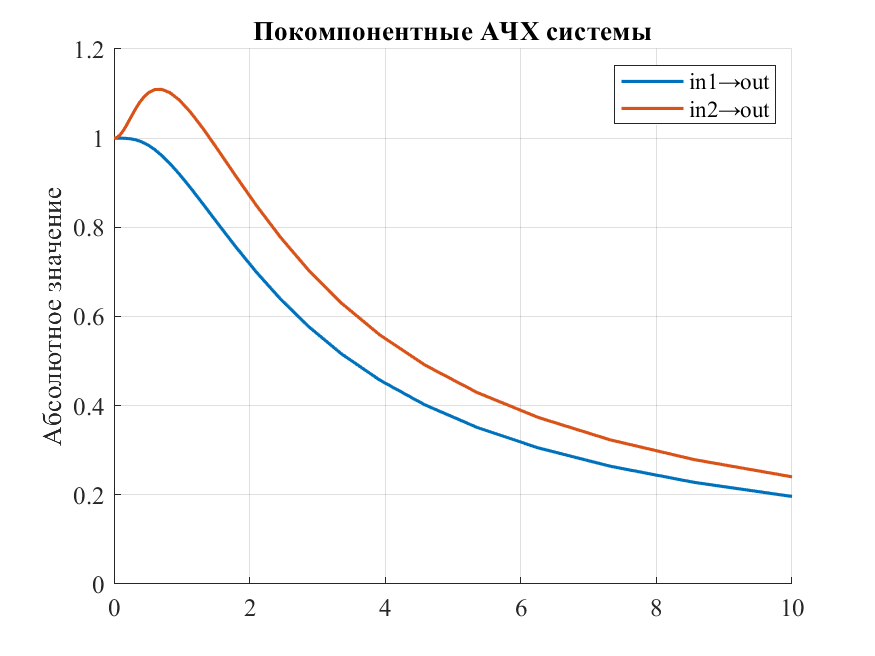
\includegraphics[width=0.8\textwidth]{freq_ampl_components5.png}
    \caption{Покомпонентные АЧХ}
  \end{figure}
\begin{figure}[ht]
  \centering
  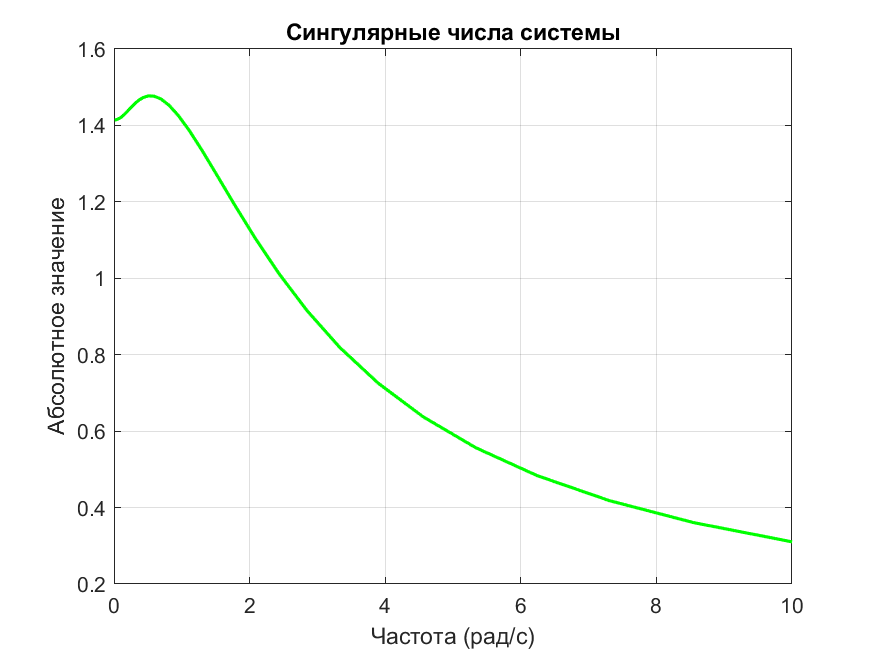
\includegraphics[width=0.8\textwidth]{singular_values5.png}
  \caption{Сингулярные числа}
\end{figure}

$$
    ||W||_{\mathcal{H}_2} \approx 1.56
$$

$$
    ||W||_{\mathcal{H}_\infty} 1.47
$$

Выберем хорошую и плохую частоту $f_1, f_2$. 
Хорошей частотой для нас будет являться та, которая меньше увеличивает сигнал по амплитуде, и наоборот.
$$
    f_1 = 7 \text{Hz}, \tab f_2 = 0.5 \text{Hz}
$$

\newpage
\subsection{Первое гармоническое возмушение}
\begin{figure}[ht]
    \centering
    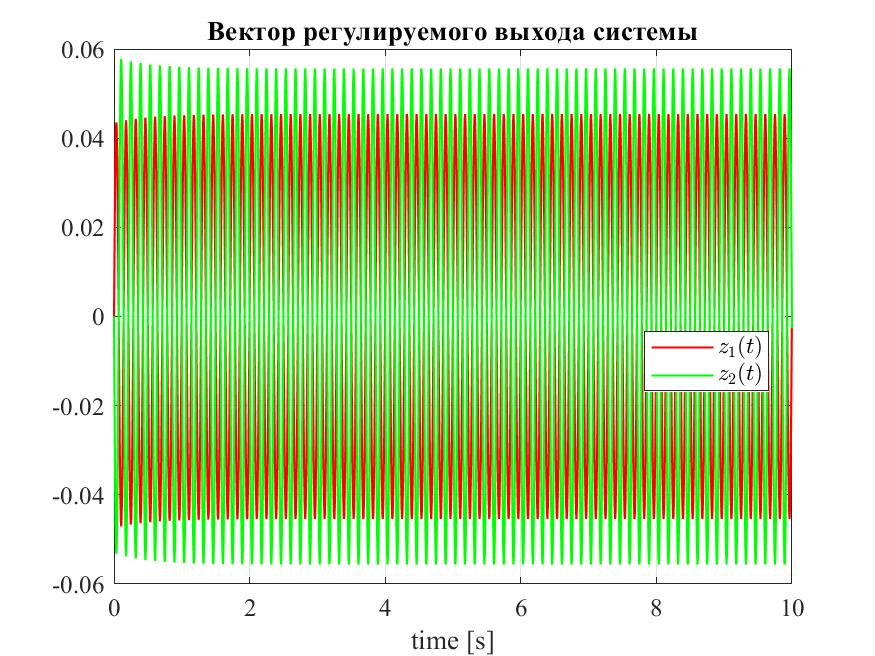
\includegraphics[width=0.8\textwidth]{z9.png}
    \caption{Моделирование -  регулируемый выход $z(t)$}
  \end{figure}
\newpage
\subsection{Второе гармоническое возмушение}
\begin{figure}[ht]
    \centering
    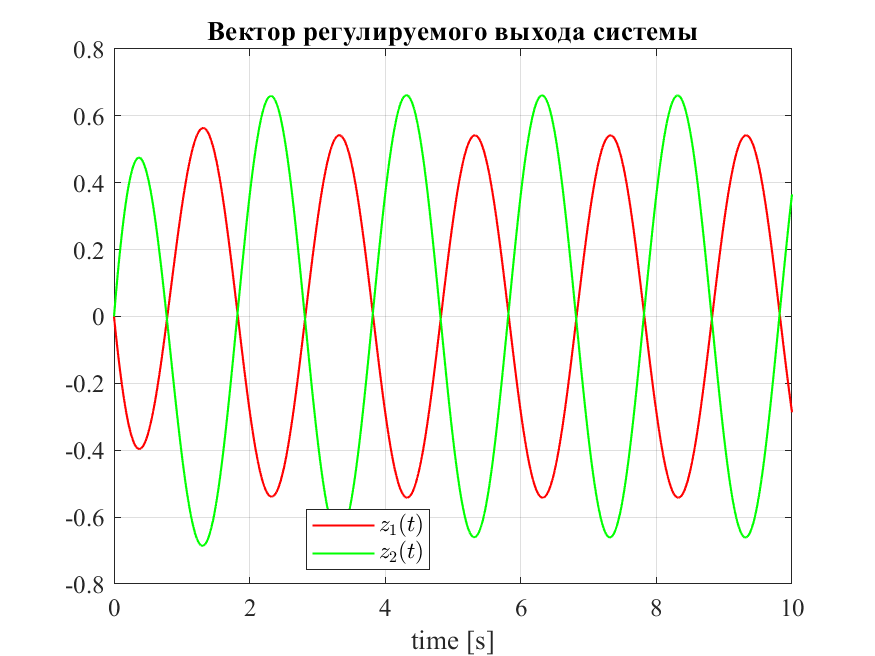
\includegraphics[width=0.8\textwidth]{z10.png}
    \caption{Моделирование -  регулируемый выход $z(t)$}
  \end{figure}


Теперь для сравнения, минимизируем вручную параметр "итеративно", пока система будет иметь решения.

В моём случае мне удалось снизить до $\gamma = 1.5$, матрица регулятора: 
$$
    K = \begin{bmatrix}
        -1.34 & -3.47 \\
    \end{bmatrix}
$$
Передаточная матрица системы:
$$
    W_{w\rightarrow z}(s) = \begin{bmatrix}\frac{2s^{3} + 7.94s^{2} + 6.15s + 1.34}{1s^{4} + 6.94s^{3} + 14.71s^{2} + 9.31s + 1.8} & \frac{-3.47s^{3} - 13.37s^{2} - 9.31s - 1.8}{1s^{4} + 6.94s^{3} + 14.71s^{2} + 9.31s + 1.8} \end{bmatrix}^T
$$

Построим для $W_{w\rightarrow z}(s)$ графики покомпонентных АЧХ:
\begin{figure}[ht]
    \centering
    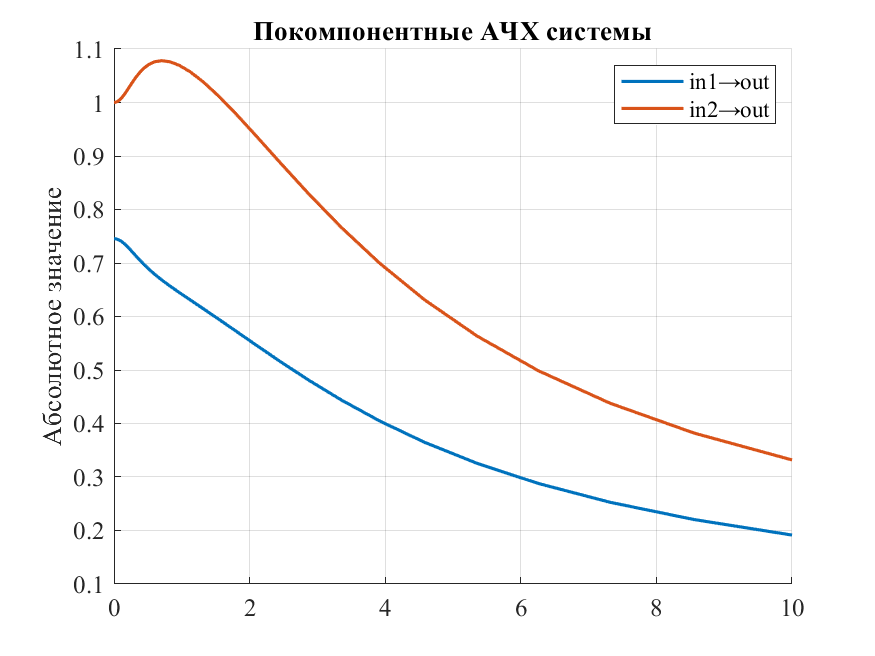
\includegraphics[width=0.8\textwidth]{freq_ampl_components6.png}
    \caption{Покомпонентные АЧХ}
  \end{figure}
Теперь построим для $W_{w\rightarrow z}(s)$ график сингулярных чисел:
\begin{figure}[ht]
  \centering
  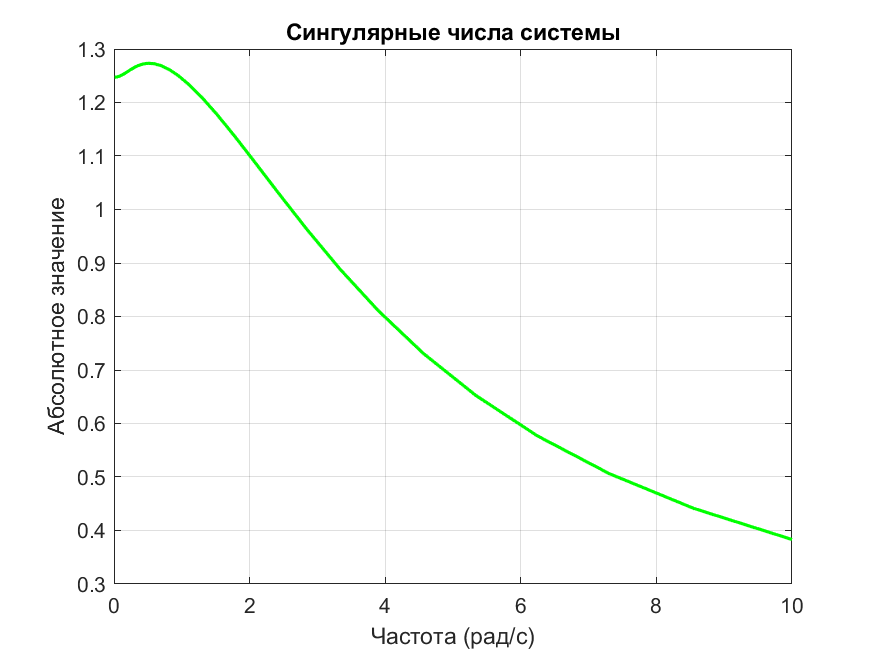
\includegraphics[width=0.8\textwidth]{singular_values6.png}
  \caption{Сингулярные числа}
\end{figure}
Нормы будем считать по следующим лекционным формулам, однако в \text{MATLAB} 
есть готовые реализации через функцию \text{norm}:
$$
    ||W||_{\mathcal{H}_2} \approx 1.61
$$

$$
    ||W||_{\mathcal{H}_\infty} 1.27
$$

Выберем хорошую и плохую частоту $f_1, f_2$. 
Хорошей частотой для нас будет являться та, которая меньше увеличивает сигнал по амплитуде, и наоборот.
$$
    f_1 = 7 \text{Hz}, \tab f_2 = 0.7 \text{Hz}
$$

\newpage
\subsection{Первое гармоническое возмушение}
\begin{figure}[ht]
    \centering
    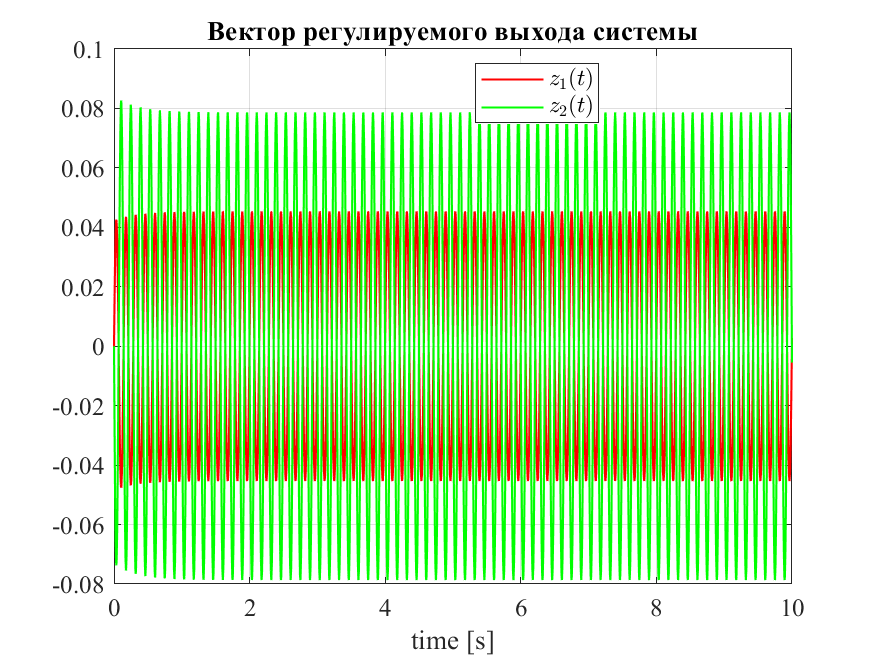
\includegraphics[width=0.8\textwidth]{z11.png}
    \caption{Моделирование -  регулируемый выход $z(t)$}
  \end{figure}
\newpage
\subsection{Второе гармоническое возмушение}
\begin{figure}[ht]
    \centering
    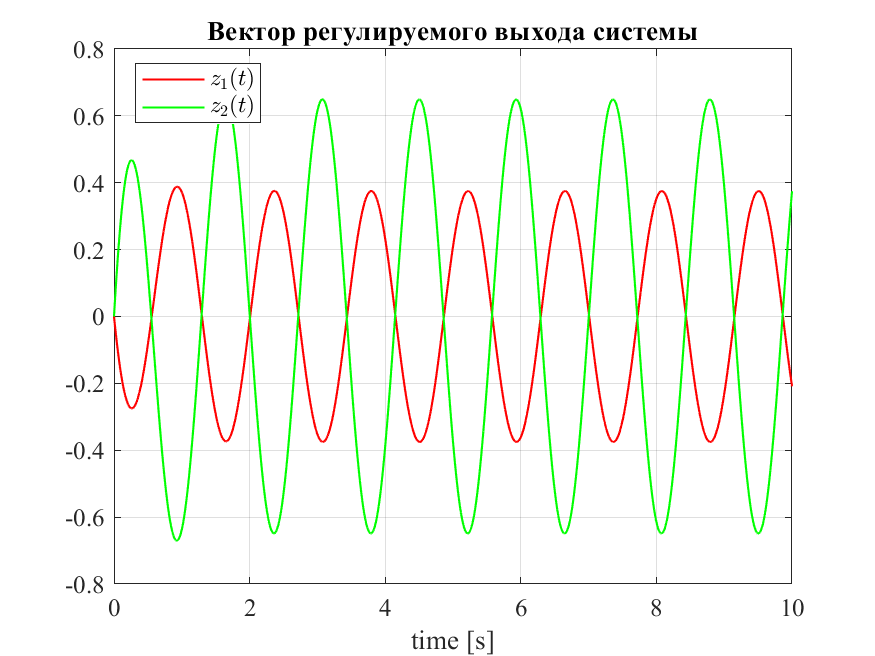
\includegraphics[width=0.8\textwidth]{z12.png}
    \caption{Моделирование -  регулируемый выход $z(t)$}
  \end{figure}

Сделаем промежуточные выводы, при минимизации $\gamma$ мы действительно получили мЕньшую  $\mathcal{H}_\infty$-норму, потому что
при дальнейший попытках понижения $\gamma$ - уравнения Риккати уже не имеют решения. При этом любопытно, что $\mathcal{H}_2$-норма ведёт себя произвольным образом, 
это и понятно - синтезированный нами регулятор отвечает за минимазацию только пиков на АЧХ. 

Здесь же и видно - теперь при попытке выбрать "плохую" частоту, итоговая амплитуда $z(t)$ будет выходить много меньше, 
чем при аналогичном случае, но с $\mathcal{H}_2$-регулятором, причины упоминались выше.

\subsection{Вывод}

В этом задании мы синтезировали $\mathcal{H}_\infty$-регулятор по состоянию, который нам позволил 
сосредоточиться на пиках АЧХ передаточной матриц системы и уменьшать амплитуду $z(t)$ именно там. 
Мы смогли удостовериться в этом при помощи моделирования.

\endinput